\documentclass[12pt]{article}

\usepackage{pgfplots}
\pgfplotsset{compat=1.18} % Or adjust depending on your TeX distribution
\usepackage[utf8]{inputenc}	% Para caracteres en español
\usepackage{amsmath,amsthm,amsfonts,amssymb,amscd}
\usepackage{multirow,booktabs}
\usepackage[table]{xcolor}
\usepackage{fullpage}
\usepackage{lastpage}
\usepackage{newtxtext}
\usepackage{newtxmath}
\usepackage{enumitem}
\usepackage{fancyhdr}
\usepackage{mathrsfs}
\usepackage{wrapfig}
\usepackage{setspace}
\usepackage{calc}
\usepackage{multicol}
\usepackage{cancel}
\usepackage[retainorgcmds]{IEEEtrantools}
\usepackage[margin=3cm]{geometry}
\usepackage{amsmath}
\newlength{\tabcont}
\setlength{\parindent}{0.0in}
\setlength{\parskip}{0.05in}
\usepackage{empheq}
\usepackage{framed}
\usepackage[most]{tcolorbox}
\usepackage{xcolor}
\usepackage{fancyvrb}
\colorlet{shadecolor}{orange!15}
\parindent 0in
\parskip 12pt
\geometry{margin=1in, headsep=0.25in}
\theoremstyle{definition}
\newtheorem{defn}{Definition}
\newtheorem{reg}{Rule}
\newtheorem{exer}{Exercise}
\newtheorem{note}{Note}
\newtheorem{theorem}{Theorem}
\setcounter{section}{0}
\usepackage{chngcntr}
\usepackage{hyperref}
\counterwithin*{equation}{section}
\counterwithin*{equation}{subsection}
\usepackage{tikz}
\usetikzlibrary{arrows.meta, positioning}
\usetikzlibrary{positioning,arrows}




\definecolor{mGreen}{rgb}{0,0.6,0}
\definecolor{mGray}{rgb}{0.5,0.5,0.5}
\definecolor{mPurple}{rgb}{0.58,0,0.82}
\definecolor{backgroundColour}{rgb}{0.95,0.95,0.92}

\lstdefinestyle{CStyle}{
    backgroundcolor=\color{backgroundColour},   
    commentstyle=\color{mGreen},
    keywordstyle=\color{blue},
    numberstyle=\tiny\color{mGray},
    stringstyle=\color{mPurple},
    basicstyle=\footnotesize,
    breakatwhitespace=false,         
    breaklines=true,                 
    captionpos=b,                    
    keepspaces=true,                 
    numbers=left,                    
    numbersep=5pt,                  
    showspaces=false,                
    showstringspaces=false,
    showtabs=false,                  
    tabsize=2,
    language=C
}

\begin{document}

\section{Introducción a los sistemas operativos}

Un programa en ejecución toma una instrucción en memoria, la decodifica, y la
ejecuta. Una vez esto se realiza, el procesador se mueve a la próxima
instrucción, y así sucesivamente. Este es el modelo de Von Neumann. 

El \textbf{sistema operativo} (SO) es un cuerpo de softwares que facilitan la ejecución
de programas, permitiéndoles compartir memoria, interactuar con dispositivos, y
simular su ejecución simultánea. La técnica principal que permite conseguir esto
se llama \textbf{virtualización}. 

La virtualización es una técnica general que permita tomar un recurso físico y
transformarlo en una representación virtual más'general, poderosa y fácil de
utilizar.  

\begin{shaded}
    \textbf{($\dagger$) Problema central.} ¿Cómo pueden virtualizarse los recursos? Es
    decir, ¿qué políticas y mecanismos debe implementar el SO para alcanzar la
    virtualización?
\end{shaded}

El sistema operativo provee interfaces (APIs) para que los usuarios se
comuniquen con él y le den instrucciones. Entre otras cosas, provee 
\textbf{llamadas a sistema} que están disponibles para las aplicaciones. 

Finalmente, el sistema operatitvo es un \textbf{administrador de recursos}, 
decidiendo de manera eficiente y justa cómo deben utilizarse los recursos
principales (CPU, memoria, y disco).


\subsection{Virtualización de la CPU}

La virtualización de la CPU consiste en la simulación de múltiples CPUs con una
sola (o pocas). En términos prácticos, esto significa simular que múltiples
programas se ejecutan simultáneamente.

\begin{shaded}

    $(\dagger)$ Considere el siguiente código.
    
\begin{verbatim}
# code name: cpu_virt.c
#include <stdio.h>
#include <unistd.h>

int main(int argc, char *argv[]) {
    if (argc < 2) {
        fprintf(stderr, "Usage: %s <string>\n", argv[0]);
        return 1;
    }

    char *msg = argv[1];

    while (1) {
        printf("%s ", msg);
        fflush(stdout);   // flush so it prints immediately
        usleep(100000);   // sleep 0.1s to let the scheduler switch
    }

    return 0;
}
\end{verbatim}

Si ejecutamos \texttt{./cpu\_virt a & ./cpu\_virt b & ./cpu\_virt c  },
esperaríamos que el primer programa nunca deje que los demás se ejecuten (pues
nunca termina). Sin embargo, se imprime primero $a$, después $b$, después $c$, y
luego se repite indefinidamente. ¿Qué impide que el primer programa monopolize
la CPU? Su virtualización.
\end{shaded}

La virtualización de la CPU trae problemas de política. Si dos programas quieren
ejecutarse al mismo tiempo, ¿cuál priorizar?  

\subsection{Virtualización de la memoria}

El modelo de la memoria es simple. La memoria es una \textit{array} de bytes.
Para leerla, uno debe espeficiar una dirección en la array. Para escribir, 
se especifica una dirección y la información que desea escribirse. 

Imaginemos un programa que ejecuta \texttt{malloc}, guarando el valor entero $0$
en la dirección de memoria $p$, e imprimiendo $p$. Imaginemos que inmediatamente
después, el programa entra en un loop y actualiza el valor de la dirección $p$
incrementándolo por uno, e imprime el valor resultante. El resultado de ejecutar
el programa será la impresión de 1, 2, 3, etc.

Ahora, imaginemos que ejecutamos este programa dos veces, "al mismo tiempo". 
Creeríamos que $p$, la dirección de memoria de cada instancia del programa,
sería diferente. Pero es la misma. Más aún, los programas no sobreescriben la
dirección de memoria a la que accede el otro. Es decir, veremos impreso: 1 1 2 2
3 3 etc. Si la dirección $p$ es la misma, ¿por qué los programas no se pisan? 

La razón es que el SO virtualiza la memoria. Cada proceso accede a su propio
\textbf{espacio virtual de direcciones}, que el OS se encarga de mapear a
direcciones de memoria física. Una referencia dentro de un programa no afecta el
espacio de memoria de otro programa. Hasta donde el programa sabe, él tiene su
propia memoria física. 

\subsection{Concurrencia}

El término concurrencia refiere un conjunto de problemas que surgen cuando
un único programa opera sobre múltiples recursos concurrentemente. El SO es el
principal ejemplo: es un conjunto de programas que manipula al mismo tiempo
múltiples cosas. Pero el problema de la concurrencia no se limita al SO: muchos
programas \textit{multi-threaded} muestran problemas similares.

\pagebreak

\section{El proceso (¿de Kafka?)}

Una de las formas fundamentales de abstracción que provee el SO es 
\textbf{el proceso}. Un proceso es un programa en ejecución. El programa en sí
es algo muerto: instrucciones en memoria, tal vez data estátitca. Es el sistema
operativo quien insufla vida.

\begin{shaded}
    $(\dagger)$ \textbf{Problema central.} ¿Cómo virtualizar la CPU?
\end{shaded}

El SO virtualiza la CPU ejecutando un proceso, deteniéndolo para ejecutar otro,
y así sucesivamente. Esta técnica se llama \textbf{time sharing} de la CPU. El
costo potencial es eficiencia, pues los programas tardarán más en terminar si la
CPU debe compartirse.

Para implementar sus funcionalidades, el SO necesita operar en el bajo bajo y
en el alto nivel. Las operaciones de bajo nivel se llaman \textbf{mecanismos}.
\textbf{Time sharing} es un mecanismos. 

Por encima de los mecanismos, hay \textbf{políticas}. Las políticas son
algoritmos que toman decisiones dentro del SO.

\subsection{Estado de máquina (machine state)}

Para entender un proceso, hay que entender qué es el estado de la máquina. 
El estado de la máquina es lo que un programa puede leer o actualizar mientras
se ejecuta. En un momento dado, ¿qué partes de la máquina importan para la
ejecución de un programa? 

El espacio de memoria, con sus instrucciones y datos, es parte del estado de
máquina. Contiene algunos registros especiales, como el program counter (PC),
también llamado instruction pointer (IP), que nos dice qué instrucción del
programa se ejecutará en el instante siguiente. Similarmente, está el stack
pointer y el frame pointer asociado, que sirven para administrar el stack con
las variables, parámetros de funciones, y return addresses. 

\subsection{API de procesos}

Todo SO moderno provee las siguientes APIs:

\begin{itemize}
    \item \textbf{Crear}. El SO debe permitir la creación de procesos nuevos. 
    \item \textbf{Destruir}. El SO debe permitir la destrucción de procesos. 
    \item \textbf{Espera}. El SO debe poder esperar que un proceso termine. 
    \item \textbf{Control misceláneo.} Controles varios, como suspender un
        proceso para resumirlo después. 
    \item \textbf{Status.} El SO debe dar una interfaz para obtener información
        acerca del estado de un proceso: hace cuánto se ejecuta, por ejemplo.
\end{itemize}


\subsection{Creación de procesos}

¿Cómo se transforma un programa en un proceso? El SO carga su código y cualquier
información estática necesaria desde el disco en la memoria virtual. Esto suele
hacerse \textit{lazily}: se van cargando en la memoria las partes a medida que
se las van necesitando en la ejecución. Luego el SO aloca memoria para el stack del
programa, donde residen las variables locales, parámetros de funciones, y
direcciones de retorno. El SO también aloca memoria para el heap, donde reside
la información dinámica (lo alocado y liberado por \texttt{malloc} y
\texttt{free}, por ejemplo). Aquí viven las estructuras de datos como arrays,
árboles, etc. 

El SO también se encarga de otras tareas de inicialización, en particular
relativas al input/output (I/O). Por ejemplo, cada proceso tiene tres
\textbf{file descriptors}: \texttt{stidin, stdout, stderr}. Éstos permiten al
programa leer input e imprimirlo o dirigirlo a alguna fuente.

Sólo después de todo esto, el SO comienza la ejecución, iniciando el programa
desde su entry point (i.e. \texttt{main()}). Una vez "salta" a la rutina
\texttt{main()}, el SO transfiere control de la CPU al proceso recién creado, y
el programa comienza.

\subsection{Estados de procesos}

Un proceso puede estar en uno de los siguientes estados: 

\begin{itemize}
    \item \textbf{Running:} El programa se está ejecutando.
    \item \textbf{Ready}: El programa está listo para ejecutarse.
\item \textbf{Blocked:} El programa está bloqueado, es decir a realizado algún
    tipo de operación y no puede continuar hasta que cierto evento ocurra. Por
    ejemplo, solicitó I/O en el disco y se bloquea hasta que la operación de I/O
    termine.
\end{itemize}

Cuando un programa pasa de \textbf{Running} a \textbf{Ready}, decimos que fue 
\textit{descheduled}. En la transición inversa, decimos que fue
\textit{scheduled}.

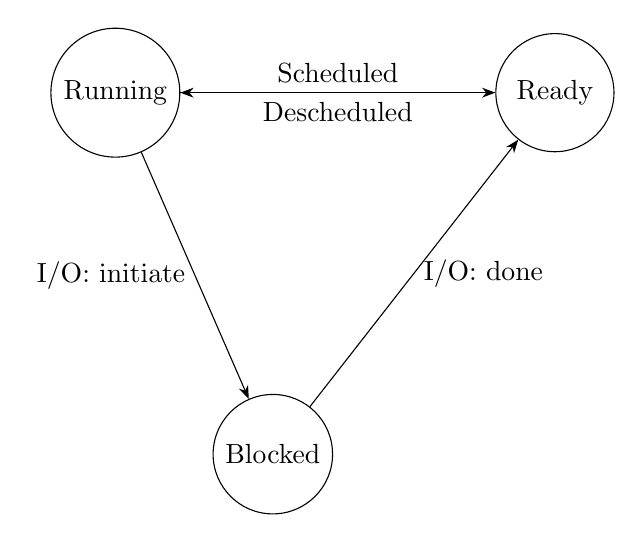
\begin{tikzpicture}[
    state/.style={circle, draw, minimum size=1.5cm},
    >=Stealth
]

% Nodes
\node[state] (running) {Running};
\node[state, right=4cm of running] (ready) {Ready};
\node[state, below=3cm of running, xshift=2cm] (blocked) {Blocked};

% Arrows between running and ready
\draw[->] (running) -- (ready) node[midway, above] {Scheduled};
\draw[->] (ready) -- (running) node[midway, below] {Descheduled};

% Arrows for I/O transitions
\draw[->] (running) -- (blocked) node[midway, left] {I/O: initiate};
\draw[->] (blocked) -- (ready) node[midway, right] {I/O: done};

\end{tikzpicture}

La parte del SO que se encarga de administrar estas transiciones de estado en
los distintos programas se llama \textbf{OS scheduler}.

A veces un proceso está en estados que llamamos \textbf{inicial} y
\textbf{final}, los estados resultanates justo cuando es creado y justo cuando
termina, respectivamente. Cuando un proceso termina pero aún no fue destruido,
decimos que está en \textbf{estado zombie}. El estado zombie permite que otros
procesos (como el proceso padre) examinen el código de retorno del proceso que
terminó y ver si se ejecutó con éxito.

\subsection{Estructuras de datos del SO}

El SO es un programa con sus propias estructuras de datos. Entre ellas,
destacarmemos las siguientes. 

El SO tiene una \textbf{lista de procesos}, con todos los procesos que están en
estado \textit{ready} y alguna información adicional para registrar cuál se está
ejecutando. El SO también lleva algún registro de los procesos bloqueados. 

El SO también tiene, para cada proceso bloqueado, un \textbf{register context}.
Dicho registro guarda el contenido de los registros del proceso bloqueado.  Así,
al resumir el proceso, sus registros pueden restaurarse.

\pagebreak 

\section{API de procesos}


\subsection{La llamada a sistema \texttt{fork()}}


Todo proceso tiene un \textbf{PID} (process identifier) y un \textit{process
group ID} (PGID). El ID identifica al proceso, y el PGID se usa para identificar
procesos que están relacionados (e.g. los procesos hijos heredan el PGID del
padre).


. La llamda a sistema
\texttt{fork()} se utiliza para crear un proceso nuevo, pero de una forma un tanto
bizarra. 

\texttt{fork()} crea una copia \textit{casi} exacta del proceso dentro del cual
ocurre la llamada. Dicha copia se llama \textit{proceso hijo}, y el proceso que
dentro del cual se llamó \texttt{fork()} se llama \textit{proceso padre}. La
ejecución del proceso hijo no comienza en el entry point \texttt{main()}, sino
justo donde la llamada a \texttt{fork()} termina.

El hijo no es una copia exacta por dos razones. Por un lado, tiene su propio
espacio de direcciones, sus propios registros, su propio PC, etc. Por otro lado,
la llamada a \texttt{fork()} en el padre devuelve el PID del proceso hijo (un
\texttt{int}). Por otro lado, en el hijo la llamada a \texttt{fork()} devuelve
\texttt{0} si el proceso se creó con éxito, y \texttt{-1} de otro modo.

\begin{shaded}
    \textbf{Ejemplo.} El siguiente código explica con comentarios lo antedicho. 

    \footnotesize
    \begin{verbatim}
#include <stdio.h>      
#include <unistd.h>    
#include <sys/types.h> 
#include <stdlib.h>    

int main() {
    // pid_t es el data type usado para representar PIDs. Suele ser un signed
    // int, aunque esto puede variar.
    pid_t pid;

    // Crea un proceso hijo. En esta línea empieza el hijo, 
    // y el valor de pid diferirá en padre e hijo.
    pid = fork();  

    if (pid < 0) {
        perror("fork failed");
        exit(1);
    }
    else if (pid == 0) {
        printf("Child process: PID = %d, Parent PID = %d\n", getpid(), getppid());
    }
    else {
        printf("Parent process: PID = %d, Child PID = %d\n", getpid(), pid);
    }

    // Padre e hijo, ambos, ejecutarán la siguiente línea.
    printf("Soy ejecutado por ambos procesos. (PID = %d).\n", getpid());

    return 0;
}
    \end{verbatim}
    \normalsize
\end{shaded}

La ejecución de \texttt{fork()} es \textbf{no-determinística}: cuando se crea el
hijo, dos procesos activos (padre e hijo) compiten por la CPU, y cualquiera de
los dos puede ser ejecutado dependiendo de la decisión tomada. El
\textbf{scheduler} determinará quién se ejecuta primero, pero esto no podemos
determinarlo de antemano.

\subsection{La llamada a sistema \texttt{wait()}}

Generalmente, es útil pausar el proceso padre hasta que el proceso hijo termine.
Esto puede hacerse con \texttt{wait()}. La llamada a \texttt{wait()} combinada
con \texttt{fork()} hace que \texttt{fork()} sea determinístico.

En la práctica, \texttt{wait()} tiene dos comandos asociados, \texttt{waitpid()}
y \texttt{waitid()}.  Todos estos comandos se usan para esperar un
\textbf{cambio de estado} en un proceso hijo (el hijo terminó, fue interrumpido
por una señal, fue resumido por una señal). Cuando un hijo termina, es la
llamada a \texttt{wait()} lo que permite liberar los recursos asociados al hijo;
de otro modo, el hijo quedaría en un estado zombie.

La llamada \texttt{waitpid()} es un wrapper sobre \texttt{wait()}. En
particular, \texttt{wait()} tiene la siguiente signature:

\begin{equation*}
    \texttt{pid\_t wait(int *\_Nullable wstatus)}
\end{equation*}

\texttt{wstatus} es un puntero a un \texttt{int}, y se corresponde con la
dirección de memoria donde se escribirá qué sucedió con el proceso hijo. En
general, en \texttt{wstatus} se escribe la PID del proceso hijo cuando el mismo
terminó con éxito, y se escribe \texttt{-1} si hubo un error. El puntero
\texttt{wstatus} puede ser nulo (de allí el \texttt{\_Nullable}), lo cual
significa: "no me importa qué suceda con el proceso hijo".

La llamada \texttt{waitpid()} tiene la siguiente signatura:

\begin{equation*}
    \texttt{pid\_t waitpid(pid\_t pid, int *\_Nullable wstatus, int options)}
\end{equation*}

Esta llamada suspende la ejecución hasta que el proceso hijo con PID
\texttt{pid} cambie de estado. Por defecto, \texttt{waitpid()} espera solo
terminaciones y no otros cambios de estado, como interrupciones. Este
comportamiento se puede modificar vía el argumento \texttt{options}. 

El argument \texttt{pid} puede tomar los siguientes valores:

\begin{itemize}
    \item Valores menores a \texttt{-1}: Espera a cualquier proceso con PGID
        idéntico al valor absoluto de \texttt{pid}.
    \item \texttt{-1}: Espera por cualquier proceso hijo. 
    \item \texttt{0}: Espera a cualquier proceso cuyo PGID es idéntico al del
        proceso llamador, \textit{en el momento en que se llamó}
        \texttt{waitpid()}.
    \item Valores mayores a \texttt{0}: Espera por el proceso hijo cuyo PID es
        exactamente igual al valor de \texttt{pid}.
\end{itemize}

Como los hijos heredan el PGID del padre, pareciera que las opciones \texttt{<-1}
y \texttt{=-1} son idénticas. Pero el PGID de un proceso puede cambiarse. Por
ejemplo, un proceso puede tener dos hijos, uno de los cuales es asignado en
algún momento un PGID diferente (ver \texttt{setpgid()}). Entonces,
\texttt{waitpid(-1, ...)} esperará a cualquiera de los hijos, mientras que 
\texttt{waitpid(-2, ...)} esperará solo al que sigue teniendo una PGID idéntica
a la del padre (en valor absoluto).

El valor de \texttt{options} es un \texttt{OR} de cero o más constantes, entre
las cuales contamos: \texttt{WNOHANG}, que retorna inmediatamente si ningún hijo
ha exited (?), \texttt{WUNTRACED}, que también retorna si un hijo se ha detenido
(no terminado), y \texttt{WCONTINUED}, que también retorna si un hijo detenido
ha sido resumido. Más info en \texttt{man wait}.

Notar que si \texttt{wstatus} es un \texttt{int},

\begin{equation*}
    \texttt{wait(&wstatus)} \equiv \texttt{waitpid(-1, &wstatus, 0)}
\end{equation*}

Es decir, \texttt{wait(&status)} expresa: Esperá por cualquier proceso hijo
(\texttt{pid = - 1}), guardá la información de la espera en \texttt{wstatus},
sin ninguna flag en particular (\texttt{options = 0}).

\subsection{La llamada a sistema \texttt{exec()}}

La llamada \texttt{exec()} permite ejecutar, desde un proceso llamador, un
programa diferente al mismo. En realidad, \texttt{exec} es parte de una familia
de programas: \texttt{execl, execlp, execle,} etc. Veremos en particular 
\texttt{execv, execvp}.

La familia de programas \texttt{exec()} \textit{reemplaza} la \textbf{imagen}
del proceso actual por una nueva.

\begin{shaded}
    $(\clubsuit)$ La \textbf{imagen} de un proceso es el estado total de un
    proceso en memoria: su código, sus variables, su heap, su stack,  sus file
    descriptors, etc.
\end{shaded}

Cuando se llama \texttt{exec()} exitosamente, el proceso ya no corre su código
viejo, sino que se convierte en el programa a ejecutar. El PID permanece
idéntico, los file descriptors siguien abiertos, pero la memoria, el stack, y el
código son reemplazados. Por esta razón, \texttt{exec()} suele usarse después de
\texttt{fork()}, transformando el proceso hijo en un nuevo programa, y lograndoo
así ejecutar programas nuevos desde un programa padre.

\pagebreak 

\section{Ejecución directa limitada}

La ejecución directa de los programas no es deseable. Si la CPU ejecuta un
programa de manera directa y libre, ¿cómo garantizar que el programa no haga
algo indeseado? ¿Cómo lo detenemos, o cómo implementamos \textbf{time sharing},
si el programa tiene control de la CPU? 

La ejecución directta, por ende, debe limitarse. Llamamos al paradigma de
ejecución resultante \textbf{ejecución directa limitada}. 

\subsection{Problema 1: Restricción de operaciones}

La ejecución directa tiene como ventaja ser rápida: el programa corre
nativamente en la CPU (hardware). El primer problema que debemos enfrentar, sin
embargo, es permitir que el programa pueda realizar operaciones restringidas,
como I/O, sin tener control completo de la CPU. 

La solución es introducre dos \textbf{modos de procesador}: \textit{user mode} y
\textit{kernel mode}. El primero es restringido, mientras el segundo es
privilegiado. 

Cuando un programa desea realizar una operación privilegiada, como leer del
disco, se utiliza una \textbf{llamada a sistema}. Las llamadas a sistema
permiten que el \textit{kernel} exporte ciertas funcionalidades esenciales a
los programas del usuario, como acceder a un archivo del sistema, crear y
destruir procesos, alocar memoria, etc. 

Para ejecutar una llamada a sistema, el programa jecuta una \textbf{trap
instruction}. Esta instrucción simultáneamente salta al kernel y eleva el nivel
de privilegio al \textit{kernel mode}. Una vez en este estado, el sistema puede
realizar la operación privilegiada deseada. Al terminar, el SO ejecuta una
\textbf{return-from-trap instruction}, que vuelve al programa original y a la
vez reestablece el \textit{user mode}.

Al realizar la \textbf{trap instruction}, el procesador guarda en el
\textbf{kernel stack} los registros, PC y flags del programa, a fin de
reestablecer una vez que se vuelve del kernel.

¿Cómo sabe la \textbf{trap} qué codigo ejecutar dentro del SO? El proceso no
puede decirle a qué instrucción ir, porque eso permitiría que los programas
vayan a cualquier lugar del kernel (malísimo). Por el contrario, cuando se
inicia la computadora (en kernel mode), el kernel establece una \textbf{trap
table}, informande al hardware en qué lugar de memoria residen los
\textbf{trap handlers}, i.e. las instrucciones que se encargan de ejecutar una
llamada a sistema. Por ende, cuando una \textbf{trap instruction} ocurre, el
hardware ya sabe dónde residen los \textbf{handlers}.

En particular, cada llamada sistema tiene un \textbf{system-call number}, un
identificador. El SO, cuando maneja una llamada a sistema dentro de un trap
handler, ve si el identificador es válido y, si lo es, ejecuta el código
correspondiente. Este nivel añadido de indirección provee protección: el código
de usuario no especifica a qué dirección saltar, sino que solicita un servicio a
través de un número identificador.

De este modo, la ejecución directa limitada tiene dos fases. En boot time, el
kernel inicializa la trap table y la CPU recuerda su ubicación. Luego, cuando un
proceso se ejecuta, el kernel organiza algunas cosas (alocar un nodo en la lista
de procesos, alocar memoria) y luego usa una return-from-trap instruction para
empezar la ejecución del proceso. Esto hace que la CPU pase a user mode y la
ejecución comienze. Si el proceso desea hacer una llamada a sistema, se vuelve
al SO vía una trap instruction, y el SO maneja la llamada y luego retorna al
programa vía una return-from-trap. 

\subsection{Problema 2: Cambio entre procesos}

Si un proceso se ejecuta en la CPU, por definición se sigue que el SO no se está
ejecutando. ¿Cómo puede el SO cambiar de un proceso a otro entonces? 

\subsubsection{Approach cooperativo}

Una estrategia se denomina \textbf{cooperativa}. El SO confía en que el proceso
será razonable y devolverá el control eventualmente para que el SO decida cómo
continuar. Esto suele hacerse mediante una llamda especial, i.e. \textbf{yield}.
También se asume que se devuelve el control al SO cuando se hace una operación
ilegal (e.g. div. por cero o acceder a memoria privilegiada). En esta
estrategia, entonces, el SO retoma control porque los programas lo ceden.

Problema obvio: programas maliciosos, loops infinitos, etc.

\subsubsection{Approach no cooperativo}

La pregunta central es cómo puede el SO retomar control sin cooperación de los
programas. La respuesta es simple: se usa un \textbf{timer interrupt}, es decir
un contador que llama una interrupción cada $k$ milisegundos. Cuando una
interrupción se llama, un \textbf{interrupt handler} pre-configurado en el SO
toma control, y el SO decide qué hacer. El código a ejecutar cuando se produce
el timer interrupt se define en boot time, donde también se inicia el timer.

\subsection{Guardando y restableciendo contextos}

Ya tenemos un sistema que permita el SO retomar control. Para decidir qué hacer
cuando el control es retomado, el SO usa un \textbf{scheduler}. Lo que nos
interesa ahora es qué sucede cuando el \textbf{scheduler} decide cambiar el
programa que se está ejecutando. 

Cuando esto sucede, el SO ejecuta un código de bajo nivel que llamaremos
\textbf{context switch}. Conceptualmente, guarda los valores de registros del
proceso actual dentro de su entrada correspondiente en el kernel stack (una por
proceso). Luego se encarga de que la return-from-trap no rediriga al proceso
actual, sino al que ahora debe ejecutarse. El kernel stack pointer se mueve al
stack de este proceso sucesor. Así, se entra al kernel en el contexto de un
proceso (el interrumpido) y se sale en el contexto de otror (el sucesor).

Notar que hay dos tipos de guardados/restablecimientos ocurriendo. El primero es
cuando ocurre el timer interrupt: los \textit{user registers} del proceso
interrumpido son guardados en el hardware, en el kernel stack de ese proceso.
Luego, el SO switchea al sucesor: los \textit{kernel registers} son guardados
por el SO en memoria, lo cual significa que ahora el sistema está en un estado
idéntico al que resultaría si hubiera realizado la trap instruction desde el
proceso sucesor. Por esto es que la return-from-trap instruction nos lleva al
sucesor, que ahora empieza a ejecutarse.



\pagebreak 


\section{Scheduling}

Scheduling se refiere a las políticas tomadas para asignar recursos
(principalmente la CPU) a los procesos que los demandan. Pueden compararse
usando métricas de performance o de justicia (fairness).

\subsection{Supuestos sobre el workload}

Al conjunto de procesos que corren en un sistema se lo denomina colectivamente
\textit{workload}. Dependiendo de los supuestos que uno haga respecto del
\textit{workload}, distinas políticas serán posibles.

Por ahora, asumimos:

\begin{enumerate}
    \item Todo proceso se ejecuta por la misma cantidad de tiempo.
    \item Todos los procesos llegan al mismo tiempo.
    \item Una vez iniciado, un proceso se ejecuta hasta termina. 
    \item Todos los procesos sólo usan la CPU (nada de I/O).
    \item El tiempo de ejecución de cada proceso es conocido \textit{a priori}.
\end{enumerate}

\subsection{Métricas}

Para comparar distintas políticas, necesitamos métricas. La primera que usaremos
se denomina \textbf{turnaround time}: 

\begin{equation*}
    T_{\text{turnaround}} = \text{T}_{\text{terminación}} - T_{\text{llegada}}
\end{equation*}

Como hemos asumido que todos los procesos llegan al mismo tiempo, por ahora el
tiempo de llegada es cero y por lo tanto el turnaround time es simplemente el
tiempo en que el proceso terminó. 

\subsection{Política FIFO}

La política FIFO es razonable bajo nuestros supuestos. Si $A, B, C$ llegan en
ese orden y al mismo tiempo $T_{\text{llegada}} = 0$, y duran cada uno $10$s, 
entonces el tiempo promedio de turnaround será 

\begin{equation*}
    \frac{\text{Turnaround}(A) + \text{Turnaround}(B) + \text{Turnaround}(C)
    }{3} = \frac{ 10 + 20 + 30 }{3} = 20
\end{equation*}

Pero si relajamos el supuesto (1) y admitimos que los procesos pueden durar una
cantidad distinta de tiempo, FIFO puede ser muy malo. Por ejemplo, si A dura
100s mientras B y C siguen durando 10, el tiempo promedio de turnaround será 
110, porque B y C (que son breves) deben esperar que A termine.

A esto se le llama \textbf{convy effect}: cierta cantidad de consumidores
relativamente breves de un recurso quedan esperando detrás de un consumidor
excesivo. 

\subsection{Shortest Job First (SJF)}

Como asumimos que los procesos llegan al mismo tiempo y que conocemos su
duración, otra política posible es ordenarlos y correr los más cortos primero
(con algún criterio arbitrario para los empates). Entonces, si A dura 100 y B, C
duran 10, el tiempo promedio de turnaround es de 50, porque 

\begin{equation*}
    \text{Turnaround}(A) = 10, \qquad \text{Turnaround}(B) = 20, \text{
    Turnaround}(C) = 120
\end{equation*}

Puede demostrarse que bajo los supuestos dados, SJF es un algoritmo de
scheduling \textbf{óptimo}. El problema es que si relajamos el supuesto (2) y
pensamos que los procesos pueden llegar en cualquier momento, tenemos
problemas. Por ejemplo, si A llega un poquito antes que B y C, otra vez
sucederá que B y C deberán esperar que A termine.

\subsection{Shortest time-to-completion first (STCF)}

Para resolver el problema, debemos relajar el supuesto (3) y permitir que los
programas puedan detenerse en vez de ejecutarse siempre hasta terminar.

Si B y C llegan después de A, la idea es que el scheduler pueda pausar A y
decidir ejecutar alguno de los otros programas, tal vez continuando A después.
Si añadimos esta facultad a SJF, tendremos STCF. Cada vez que un nuevo proceso
entra al sistema, el scheduler determina cuál de todos los procesos (incluyendo
el que está ejecutándose) tiene el menor tiempo restante, y prioriza ese. Así, 
STCF pausaría A priorizando B y C, y sólo cuando éstos terminan continuaría
corriendo A.

Por ejemplo, asumamos que A llega en $t = 0$ y B y C llegan en tiempo $t = 10$,
donde A dura 100s y los demás 10s. Los turnaround son:

\begin{enumerate}
    \item B llega en $t=10$ y termina en $t = 20$, así que su turnaround es 10. 
    \item C llega en $t = 10$ y termina en $t = 30$, su turnaround es 20. 
    \item A llega en $t = 0$ y se ejecuta por diez segundos, tras lo cual pausa
        20 segundos mientras A y B corren, y luego hace sus 80 segundos
        restantes. O sea que $A$ termina en $t = 120$ y su turnaround es 120.
\end{enumerate}

El turnaround promedio entonces es $( 20 + 30 + 120 ) / 3 = 50$. Lo cual no está
mal.


El problema con STCF es que no siempre tiene un buen tiempo de respuesta, donde 

\begin{equation*}
    \text{T}_{\text{response}} = T_{\text{firstrun}} - T_{\text{arrival}}
\end{equation*}j


El tiempo de respuesta (\textbf{response time}) es el tiempo que pasa entre el
momento en que el proceso llega y el momento en que es scheduled. Si tres
procesos llegan al mismo tiempo, el tercero debe esperar que los dos primeros
terminen en su totalidad antes de arrancar. Esto destruye la interactividad.

\subsection{Round Robin (RR)}

La idea del algoritmo de Round-Robin es no ejecutar los procesos hasta que
terminan, sino durante cierta ventana de tiempo denominada \textbf{quantum},
pasando luego al próximo programa en la cola. Hace esto repetidamente hasta que
todos los trabajos terminan. 

\begin{shaded}
    $(\dagger)$ Notar que el \textbf{quantum} debe ser un múltiplo del timer
    interrupt.
\end{shaded}

\begin{shaded}
    \textbf{Ejemplo.} Asuma que A, B, C llegan al mismo tiempo y desean correr
    por 5s. Asuma que el quantum es 1s. Entonces se ejecuta A por 1s, B por 1s,
    C por 1s, y se repite, así 5 veces. El response time de A es cero, el de B
    es 1 y el de C es 2, dando un promedio de 1. Observar que en SJF el response
    time promedio sería $(0 + 5 + 10) / 3 = 5$.

    ¿Y el turnaround time? Todos los procesos llegan en $t = 0$, y cada uno se
    ejecuta una vez cada tres segundos, necesitando cinco segundos en total para
    terminar. Por lo
    tanto, A se ejecuta en los tiempos $t_A = \left\{ 0, 3, 6, 9, 12 \right\} $, 
    B en los tiempos $t_B = \left\{ 1, 4, 7, 10, 13 \right\} $, y C en los
    tiempos $t_C = \left\{ 2, 5, 8, 11, 14 \right\} $. Por ende, A termina en el
    tiempo 13, B en el 14, y C en el 15. El promedio de turnaround time es 14:
    ¡malardo!
\end{shaded}

El quantum es crítico: cuanto menor sea, mejor la performance bajo la métrica de
response time. Sin embargo, si es muy breve, el context switch dominará la
performance. (Imagine el ejemplo extremo: un quantum menor a la duración del
context switch!)

Por eso se deseas \textbf{amortizar} el costo de hacer cambio de contexto,
encontrar un trade-off que permita rapidez sin dejar que el cambio de contexto
domine.

\subsection{Incorporando I/O}

Cuando un programa solicita una operación de I/O al kernel, pasa al estado
\textbf{blocked} esperando que termine la solicitud. El proceso puede ser
relativamente largo, y por ende el scheduler podría decidir encolar otro proceso
mientras se espera que la operación de I/O termine.

\pagebreak 

\section{Multi-level Feedback Queue}

El problema a resolver es: optimizar el \textit{tiempo de retorno} (tiempo que un proceso pasa en el sistema) mientras se minimiza el \textit{tiempo de respuesta} (logrando así interactividad), y hacerlo bajo supuestos débiles.

La \textit{cola multinivel con retroalimentación} (MLFQ) manejará varias colas distintas, cada una asignada a un \textbf{nivel de prioridad}. En todo momento, cada proceso pertenece a una y solo una cola.

\textit{Dentro de cada cola}, usamos \textit{round-robin}. Entre colas, usamos el nivel de prioridad de las colas. Así, para dos procesos $A, B$, las dos primeras reglas son:

\begin{enumerate}
\item Si $Pr(A) > Pr(B)$, A se ejecuta y B no.
\item Si $Pr(A) = Pr(B)$, entonces A y B se ejecutan en RR.
\end{enumerate}

Obviamente, si las prioridades fueran constantes, el sistema no tendría sentido.
Por ello, la prioridad de un trabajo varía según su comportamiento observado. Si
un proceso cede repetidamente la CPU mientras espera entrada desde el teclado,
su prioridad será alta. Si un proceso usa CPU intensivamente por mucho tiempo,
MLFQ reducirá su prioridad. Así, MLFQ tratará de aprender acerca de los procesos
mientras ellos corren, usando el pasado para predecir el futuro.


\subsection{Cambios de prioridad}

En el workload, tal vez hayan procesos breves e interactivos que ceden la CPU
frecuentemente, y procesos codiciosos (CPU-bound) que necesitan un uso largo de
la CPU pero no requieren interactividad.

Llamamos \textbf{allotment} a la cantidad de tiempo que un proceso puede durar
en cierta prioridad $k$ antes de que el scheduler cambie su prioridad. Por
simplicidad, asumiremos por el momento que el allotment es igual al quantum.
Un intento de algoritmo para ajustar prioridades es el siguiente: 

\begin{itemize}
    \item Cuando un proceso ingresa al sistema, se le asigna prioridad máxima. 
    \item Si usa todo su allotment mientras se ejecuta, bajamos su prioridad. 
    \item Si el proceso cede la CPU antes de su allotment, se queda en el mismo
        nivel de prioridad.
\end{itemize}

Analicemos algunos casos. Imaginemos un único proceso codicios que dura en un
sistema con un quantum (y por ende un allotment) de 10ms. Imaginemos que hay
tres queues de prioidad. El proceso empieza en la más alta, baja después de un
quantum a la segunda, y baja después de otro quantum a la tercera, y permanece
en ella hasta que termina.

Ahora imaginemos dos procesos: A, codicioso y largo (100ms), y B, que es breve e
interactivo (20ms). Asumamos que A ha estado corriendo por un tiempo mayor a
20ms y ahora ingresa B al sistema. Para cuando B ingresa, A ya está
en la cola de más baja prioridad, y B es insertado en la máxima prioridad. B
hace sus primeros 10ms en la máxima prioridad, y sus últimos 10ms en la segunda
prioridad, y nunca llega a la más baja. Cuando B termina, A vuelve a comenzar.

\begin{shaded}
    $(\dagger)$ Fijate lo que hace MLFQ en ese último ejemplo: no sabe si B, al
    ingresar, es breve o no, pero asume que lo es. Si no lo es, irá bajando su
    prioridad. En este sentido, MLFQ se aproxima a SJF.
\end{shaded}

Imaginemos ahora un proceso B con I/O. Una regla es que si un proceso cede la
CPU antes de su allotment, queda en la misma prioridad. Imaginemos que B es
breve e interactivo, y un proceso A codicioso y largo se estuvo ejecutando hace
rato cuando B entra al sistema. A ya está en la última cola, y cuando B ingresa
en máxima prioridad toma la CPU y la cede antes del allotment. B sigue haciendo
esto, y queda siempre en la máxima prioridad, y A se ejecuta sólo en los
espacios de tiempo en los que B cede la CPU. Así, MLFQ logra interactividad y
eficiencia.


\subsection{El boost de prioridades}

Las reglas presentadas antes tienen problemas. Uno de ellos es
\textbf{starvation}: si hay demasiados procesos breves e interactivos, los
codiciosos y largos nunca recibirán la CPU.

Otro problema es que un usuario maligno podría escribir un programa que hackee
el scheduler. Por ejemplo, un programa que justo antes del allotment haga un
llamado I/O trivial (e.g. \texttt{open} un archivo), soltando momentáneamente la
CPU. De este modo, se quedaría siempre en la máxima prioridad y tener un
porcentaje de uso de CPU mayor. Si esto se hace bien (e.g. haciendo la operación
I/O después de que pasó 99\% del tiempo de allotment), el proceso podría
monopolizar la CPU.

Por último, un programa puede cambiar su comportamiento. Un programa codicioso
puede pasar a una fase interactiva, y necesitaría poder subir de prioridad.

Para lidiar con estos problemas, añadimos una nueva regla: 

\begin{itemize}
    \item Después de cierto tiempo S, todos los procesos se mueven a la más alta
        prioridad.
\end{itemize}

Notar que esta regla resuelve el problema de \textbf{starviation}, pues todo
proceso después de una cantidad de tiempo S alcanzará máxima prioridad y
recibirá CPU según el esquema de Round-Robin. También resuelve el problema de
boostear y reorganizar prioridades. El único problema que falta resolver es el
hackeo. 

Este problema se hace \textit{acumulando} el allotment time. Es decir,
descendemos un proceso si ha usado su allotment, independientemente de si lo usó
en una sola ejecución corrida o en una ráfaga de varias ejecuciones distintas. 

\subsection{Resumen de las reglas}

La MLFQ final usa las siguientes reglas: 

\begin{enumerate}
    \item Si la prioridad de A es mayor a la de B, ejecutar A. 
    \item Si tienen la misma prioridad, usar Round-Robing en la cola. 
    \item Cuando un proceso entra, se le asigna máxima prioridad. 
    \item Cuando un proceso usa todo su allotment (no importa cuántas veces haya
        cedido la CPU), se reduce su prioridad. 
    \item Después de un periodo de tiempo $S$, todos los procesos son lifteados
        a la máxima prioridad.
\end{enumerate}









































\pagebreak
\section{Ejercicios: Mecanismos}

\begin{shaded}
    
\textbf{(1)} En un sistema operativo que implementa procesos se ejecutan instancias del proceso \texttt{pi} que computa los dígitos de $\pi$ con precisión arbitraria.

\begin{verbatim}
$ time pi 1000000 > /dev/null & ... & time pi 1000000 > /dev/null &
\end{verbatim}

Y se registran los siguientes resultados, donde en las mediciones se muestra \textit{(real, user)}, es decir el tiempo del reloj de la pared (walltime) y el tiempo que insumió de CPU (cputime).

\begin{center}
\begin{tabular}{|c|>{\raggedright}m{9cm}|c|}
\hline
\#Instancias & Medición & Descripción \\
\hline
1 & (2.56, 2.44) & \\
\hline
2 & (2.53, 2.42),  (2.58, 2.40) & \\
\hline
1 & (3.44, 2.41) & \\
\hline
4 & (5.12, 2.44),  (5.13, 2.44),  (5.17, 2.46),  (5.18, 2.46) & \\
\hline
3 & (3.71, 2.42),  (3.85, 2.42),  (3.86, 2.44) & \\
\hline
2 & (5.04, 2.36),  (5.09, 2.43) & \\
\hline
4 & (7.67, 2.41),  (7.67, 2.44),  (7.73, 2.44),  (7.75, 2.46) & \\
\hline
\end{tabular}
\end{center}

\begin{enumerate}
    \item[(a)] ¿Cuántos núcleos tiene el sistema?
    \item[(b)] ¿Por qué a veces el cputime es menor que el walltime?
    \item[(c)] Indique en la \textbf{Descripción} qué estaba pasando en cada medición.
\end{enumerate}



\end{shaded}


El CPU time se mantiene prácticamente constante, como es esperable. La segunda
fila indica que hay al menos $\geq 2$ cores, porque con dos procesos el CPU time
y el walltime siguen siendo aproximadamente iguales. El hecho de que un solo
proceso en la tercera medición tiene $real > user$ indica que la medición se
llevó a cabo mientras otros procesos eran ejecutados. Esto también explica que
$real > user$ en la penúltima medición.

La cuarta medición es interesante, porque con cuatro procesos tenemos $real
\approx 5s$, es decir aproximadamente el doble de lo que toma una sola instancia
aislada. Esto soporta la idea de que la máquina tiene $=2$ cores.

Bajo la misma línea, en la tecera medición, tres instancias toman $real \approx
3.80s$, es decir $\approx 1.5$ veces lo que toma una sola instancia. Esto
soporta la idea de que hay $< 3$ cores, y en particular de que hay exactamente
$2$, porque $3 / 2 = 1.5$.

\pagebreak 

\begin{shaded}
    \textbf{(2)} En un sistema operativo que implementa procesos e hilos se ejecutan el siguiente
proceso. 

\begin{verbatim}
    
$ time ./dgemm 2000 2000 2000
test!
m=2000,n=2000,k=2000,alpha=1.200000,beta=0.001000,sizeofc=4000000
real 0m1.027s
user 0m1.752s
\end{verbatim}

Explique porque ahora $wall < cpu$.


\end{shaded}

Cuando usamos $k$ hilos, el $cpu$ time se mide como 

\begin{equation*}
    \text{CPUTime} = \sum_{i=1}^k T(\text{thread}_i)
\end{equation*}

donde $T(\text{thread}_i)$ es el tiempo utilizado en el hilo $i$. Sin embargo,

\begin{equation*}
    \text{Walltime} \geq \max \left\{ T(\text{thread}_i) : 1 \leq i \leq k \right\} 
\end{equation*}

porque una vez que todos los hilos terminan se puede devolver el resultado y
terminar el proceso. Más aún, si la paralelización es buena, 

\begin{equation*}
    \text{Walltime} \approx \max \left\{ T(\text{thread}_i) : 1 \leq i \leq k \right\} 
\end{equation*}

Claramente, acá puede acontecer que $wall < cpu$. Por ejemplo, si cada hilo uno
de tres hilos toma $0.5s$, el cpu time es 1.5 pero el wall time es 0.5.

\pagebreak 

\begin{shaded}
    \textbf{(4)} Un programa define la variable \texttt{int x=100} detro de
    \texttt{main()} y hace \texttt{fork()}.
(a) ¿Cuánto vale \texttt{x} en el proceso hijo?
(b) ¿Qué le pasa a la variable cuando el proceso padre y el proceso hijo le cambian de valor?
(c) Contestar nuevamente las preguntas si el compilador genera código de máquina
colocando esta variable en un registro del microprocesador.
\end{shaded}

$(a)$ En el proceso hijo, \texttt{x} vale \texttt{100}, porque el hijo es una
copia exacta del padre excepto su PID.

$(b)$ La variable \texttt{x} cambia de valor independientemente en ambos
procesos. Si el padre la cambia, el cambio no se ve reflejado en el proceso
hijo, y viceversa. 

$(c)$ Recordemos que los registros son ubicaciones de memoria de muy rápido
acceso que están directamente en la CPU. Cuando un proceso se ejecuta, estos
registros contienen información específica de ese proceso. Cuando se produce un
context switch, los valores de los registros se guardan en el PCB (process
control block) para poder ser restaurados luego, y se reemplazan con los valores
del proceso sucesor.

Supongamos que el compilador genera código de máquina guardando la variable en
un registro especial $R$ dentro del microprocesador, que \textit{no forma parte
del contexto de cada proceso} (es decir, no se guarda ni restaura durante un
context switch).  

Bajo este supuesto hipotético:  

\begin{enumerate}
    \item Después de \texttt{fork()}, tanto el proceso padre como el hijo tienen
inicialmente \texttt{x = 100}, ya que el hijo copia el valor inicial.  
\item Si el
proceso padre cambia \texttt{x}, ese cambio se refleja inmediatamente en el
proceso hijo, y viceversa, porque ambos están accediendo al mismo registro
físico $R$.  
\item  Esto rompe el comportamiento normal de variables locales tras
\texttt{fork()}, pero es consistente con la hipótesis de un registro “fuera del
user space” que no se guarda en el PCB.  
\end{enumerate} 

\textbf{Nota:} Este escenario es puramente teórico y no ocurre en sistemas
operativos reales, donde todos los registros de usuario se guardan y restauran
durante los context switches.

\pagebreak 

\begin{shaded}
    
\textbf{(5)} Indique cuantas letras “a” imprime este programa, describiendo su
funcionamiento.

\begin{verbatim}
printf("a\n");
fork();
printf("a\n");
fork();
printf("a\n");
fork();
printf("a\n");
\end{verbatim}

Generalice a $n$ forks. Analice para $n=1$, luego para $n=2$, etc., busque la
serie y deduzca la expresión
general en función de $n$.
\end{shaded}

Hay un impresión de $a$ antes de la primer llamada a \texttt{fork()}. 

Luego se llama \texttt{fork()}, con lo cual hay un hijo y un padre, y ambos
ejecutan la segunda instrucción \texttt{print}, con lo cual se imprime $a$ dos
veces más.

Tanto el hijo como el padre que hasta ahora tenemos llegan al segundo
\texttt{fork}, con lo cual los dos generan un hijo. Esto quiere decir que ahora 
el hijo que ya existía tiene un nuevo hermano y un hijo propio, resultando en un
total de 4 procesos. Con lo cual se imprimen 4 $a$s. 

En el último fork, el padre original tiene un nuevo hijo (ya lleva tres es en
total). Su primer hijo genera un nuevo hijo (teniendo dos en total), y también
lo hace su segundo hijo (teniendo uno en total). Por otra parte, el nieto del
proceso original (el primer hijo del primer hijo) también genera un hijo nuevo.
Esto nos da:

1 (Proceso padre) + 3 (Sus tres hijos) + 3 (sus tres nietos) + 1 (su bisnieto) =
8. 

Por ende, se imprime $a$ ocho veces, y la cantidad de impresiones totales son 1
(la inicial) + 2 + 4 + 8 = 15.

\begin{figure}[ht]
  \centering
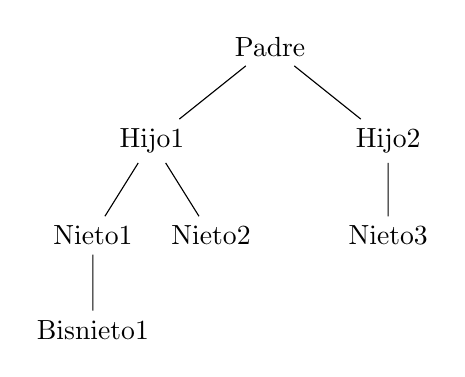
\begin{tikzpicture}[level distance=1.2cm,
  level 1/.style={sibling distance=3cm},
  level 2/.style={sibling distance=1.5cm},
  level 3/.style={sibling distance=0.75cm}]
  
\node {Padre}
  child { node {Hijo1}
    child { node {Nieto1}
      child { node {Bisnieto1} }
    }
    child { node {Nieto2} }
  }
  child { node {Hijo2}
    child { node {Nieto3} }
  };
\end{tikzpicture}
  \caption{Diagrama de procesos de tres llamadas a \texttt{fork()}}
\end{figure}

En el diagrama se hace claro que cada llamada a \texttt{fork()} agrega un nodo
hijo \textit{a todos los nodos existentes}.

Esto significa que si hay $n$ procesos (nodos), cada uno de los cuales ejecuta
\texttt{fork()}, después de dicha ejecución habrán $n$ procesos más, es decir $n
+ n = 2n$ procesos. La secuencia por ende es dada por un caso base de un proceso
y un caso inductivo de $2k$ procesos. Fácilmente se ve que esto resulta en la
regla general de $2^n$ procesos después de una llamada a fork.

Fácilmente vemos que esto coincide con la cantidad de $a$s escritas: $2^3 + 1$ ,
donde sumamos uno para contar la vez anterior a todas las llamadas de
\texttt{fork()}.

\pagebreak 

\begin{shaded}
    \textbf{(6)} Indique cuantas letras “a” imprime este programa:

    \begin{verbatim}
char * const args[] = {"/bin/date", "-R", NULL};
execv(args[0], args);
printf("a\n");
    \end{verbatim}
\end{shaded}

El programa ejecuta \texttt{date} vía \texttt{execv}. Después de la llamada a
\texttt{execv}, la imagen del proceso es reemplazada y el proceso se "convierte"
en \texttt{execv}. Por ende, la instrucción \texttt{printf("a\n")} nunca es
alcanzada. $\therefore $ El programa imprime tantas letras "a" como haya en el
output de \texttt{date}, asumiendo que \texttt{execv} no falla.

\pagebreak 

\begin{shaded}
    \textbf{(7)} Indique que hacen estos programas.

\bigskip

\noindent
\begin{minipage}[t]{0.48\textwidth}
\begin{Verbatim}[commandchars=\\\{\}]
\textcolor{red}{int} \textcolor{blue}{main}(\textcolor{red}{int} argc, \textcolor{red}{char} ** argv) \{
    \textcolor{purple}{if} (0<--argc) \{
        argv[argc] = \textcolor{red}{NULL};
        execvp(argv[0], argv);
    \}

    \textcolor{purple}{return} 0;
\}
\end{Verbatim}
\end{minipage}
\hfill
\begin{minipage}[t]{0.48\textwidth}
\begin{Verbatim}[commandchars=\\\{\}]
\textcolor{red}{int} \textcolor{blue}{main}(\textcolor{red}{int} argc, \textcolor{red}{char} ** argv) \{
    \textcolor{purple}{if} (argc<=1)
        \textcolor{purple}{return} 0;

    \textcolor{red}{int} rc = fork();
    \textcolor{purple}{if} (rc<0)
        \textcolor{purple}{return} -1;
    \textcolor{purple}{else if} (0==rc)
        \textcolor{purple}{return} 0;
    \textcolor{purple}{else} \{
        argv[argc-1] = \textcolor{red}{NULL};
        execvp(argv[0], argv);
    \}
\}
\end{Verbatim}
\end{minipage}
\end{shaded}

$(a)$ En el primer código, podríamos bien sustituir \texttt{0 < --argc} por 
\texttt{argc >= 2}, porque 

\begin{equation*}
    0 < \#\text{args} - 1 \iff 1 < \#\text{args} \iff 2 \leq \#\text{args}
\end{equation*}

Pero el Wolopriest nos quiere confundir. 

Recordemos que \texttt{argc} es la cantidad de command line arguments dados al
programa más uno (pues también cuenta el nombre del programa), y que
\texttt{argv} es una null-terminated array de \texttt{argc + 1} elementos.

Asumiendo que la condición se cumple (es decir, que al programa se le pasa al
menos un argumento), debemos notar que la línea \texttt{argv[arc] = NULL} no
hace nada, porque el último elemento de la array ya es \texttt{NULL}. Es decir
que el programa equivale a llamar \texttt{execvp(argv[0], argv)}. Por ejemplo,
si el programa se ejecuta con los arguments \texttt{ls -l}, se ejecuta el
programa \texttt{ls} con argumentos \texttt{-l}. Etc.

$(b)$ Este programa también requiere \texttt{argc >= 2} para hacer algo
efectivo. Asumamos que ese es el caso. El programa \texttt{fork}ea. Si el
\texttt{fork} falla, devuelve \texttt{-1}. Si el fork no falla, devuelve
\texttt{0} en el hijo, pero en el padre ejecuta el programa indicado por
los command line arguments con la última flag removida. (Notemos que
\texttt{argv[argc - 1] = NULL} no hace más que quitar la última flag). Para usar
el mismo ejemplo que antes, en este caso llamar el programa con \texttt{ls -l}
como command line arguments resultaría en la ejecución de \texttt{ls}.

\pagebreak 

\begin{shaded}
    \textbf{(8)} Si estos programas hacen lo mismo. ¿Para que está la syscall dup()? ¿UNIX tiene un
mal diseño de su API?

\begin{verbatim}
// Programa 1
close(STDOUT_FILENO);
open("salida.txt", O_CREAT|O_WRONLY|O_TRUNC, S_IRWXU);
printf("¡Mira mama salgo por un archivo!");
\end{verbatim}

\begin{verbatim}
// Programa 2
fd = open("salida.txt", O_CREAT|O_WRONLY|O_TRUNC, S_IRWXU);
close(STDOUT_FILENO);
dup(fd);
printf("¡Mira mama salgo por un archivo!");
\end{verbatim}

\end{shaded}

Estudiemos estos programas.

$(1)$ Recordemos que \texttt{STDOUT\_FILENO == fileno(stdout)}, es decir es el
\texttt{int} file descriptor usado para implementar el stream \texttt{stdout}
(que al ser un stream es un \texttt{FILE*} pointer). 

La primera línea cierra el file descriptor que identifica a \texttt{stdout},
después de lo cual \texttt{STDOUT\_FILENO} (que en realidad no es más que el
entero \texttt{1}) no identifica ninguna file y puede ser reusado. 

La función \texttt{open} abre el archivo \texttt{salida.txt}. La flag
\texttt{O\_CREATE} lo crea si no existe, \texttt{O\_WRONLY} es \textit{write
only}, \texttt{S\_IRWXU} no me queda claro.

La función \texttt{open} devuelve (y asigna) al archivo abierto el menor file
descriptor disponible, que al haber cerrado \texttt{1} es \texttt{1}. Por ende,
ahora 1 (es decir, \texttt{STDOUT\_FILENO}) refiere al archivo
\texttt{salida.txt}. 


\small
\begin{quote}

    \textbf{Nota.} Con "asigna", quise decir: \texttt{open} crea una entrada en
    la tabla de open files del sistema, cuyo índice es el file descriptor que
    devuelve.
\end{quote}
\normalsize

$(2)$ El segundo programa guarda en \texttt{fd} el file descriptor asignado al
archivo de salida, cierra \texttt{STDOUT\_FILENO}, y llama \texttt{dup(fd)}. 
La función \texttt{dup(fd)} toma un file descriptor abierto \texttt{fd}, y crea
un nuevo file descriptor que apunta al mismo archivo \texttt{fd}, pero es el
menor número disponible. Por lo tanto, \texttt{dup(fd)} hace que 
\texttt{1 ==STDOUT\_FILENO} apunte a \texttt{salida.txt}.

(Diferencias) En el segundo programa, \texttt{fd} y \texttt{STDOUT\_FILENO}
pueden usarse intercambiablemente, porque \texttt{fd} nunca se cierra.
\texttt{dup} permite más control porque uno puede elegir qué file descriptors
redirigir. 



\pagebreak 

\begin{shaded}
    \textbf{(10)} Para el diagrama de transición de estados de un proceso,
    describa cada uno de los cuatro escenarios posibles acerca de cómo funciona
    (o no) el SO si se quita solo una de las cuatro fechas.
\end{shaded}

El diagrama es el siguiente.

\begin{verbatim}
               

               +---------+   
               |         |  Descheduled    +---------+
               | Running | <------------>  |  Ready  |
               |         |    Scheduled    +---------+
               +---------+                       ^
                   |                             |
            I/O    |         +---------+         | I/O
          starts   |-------> | Blocked | --------| ends
                             +---------+
\end{verbatim}

Imaginemos que quitamos la transición de running a ready. ...


\pagebreak

\begin{shaded}
    \textbf{(12)} Verdadero o falso.
\end{shaded}

$(a)$ Es posible que \texttt{user + sys < real}.


\small
\begin{quote}

Recordemos que \texttt{user time} es el tiempo que la CPU ejecuta el programa en
el \texttt{user space}, es decir fuera del kernel. \texttt{sys time} es lo
opuesto: es el tiempo que el tiempo que la CPU ejecuta instrucciones del
programa \textit{kernel mode} (privilegiado), por ejemplo tras hacer una llamada
a sistema. 

\texttt{real time} es el tiempo de reloj desde el inicio de la ejecución hasta
su terminación. Incluye todo: tiempo que el programa está pausado esperando que
otros procesos se ejecuten, los tiempos que toma cada context switch, etc.

Es posible que \texttt{user + sys < real}. Por ejemplo, asuma un programa que
debe esperar 10 segundos para que termine una I/O operation, pero que la
ejecución de sus instrucciones (en kernel o user mode) dura solo 1 segundo.
Entonces $\texttt{sys} \geq 11$s, pero $\text{user + sys = 1}$.

\end{quote}
\normalsize

$(b)$ Dos procesos no pueden usar la misma dirección de memoria virtual. 


\small
\begin{quote}

Falso. Siempre y cuando dicha dirección virtual sea traducida a disttintas
direcciones de memoria física, todo bien. Es más, si se hace una \texttt{read}
operation con esa dirección, hasta puede pasar que la dirección virtual se
traduzca a la misma dirección física (i.e. dos programas leen el mismo archivo
en momentos distintos, y justo sucede que la dirección virtualizada coincide en
ambos), y en ese caso también está todo bien.

\end{quote}
\normalsize

$(c)$ 
Para guardar el estado de un proceso, es necesario salvar el valor de
todos los registros del microprocesador.


\small
\begin{quote}

Verdadero. Hay que poder restaurarlos después a todos.

\end{quote}
\normalsize

$(d)$ Un proceso puede ejecutar cualquier instrucción de la ISA.


\small
\begin{quote}

Falso. Muchas instrucciones no pueden ejecutarse directamente por un proceso.
Debe solicitar un servicio al SO para que éste haga su magia en \textit{kernel
mode}.

\end{quote}
\normalsize


$(e)$ Puede haber traps por timer sin que esto implique cambiar de contexto.


\small
\begin{quote}

Parece razonable que sí. Imaginemos el caso fantástico de un sistema en el que
un único proceso se ejecuta. Las traps por timer seguirán ejecutándose, pero el
contexto será el mismo. Lo mismo si un solo proceso está ready y running, y
todos los demás están bloqueados.

\end{quote}
\normalsize

$(f)$ \texttt{fork()} devuelve cero para el hijo porque ningún proceso tiene PID
0.


\small
\begin{quote}

Falso. Sí devuelve cero para el hijo, pero no tiene nada que ver con el hecho de
que ningún proceso tiene PID cero. Simplemente \texttt{0} codifica el éxito en
C, mientras \texttt{-1} o valores distintos a \texttt{0} codifican error.

\end{quote}
\normalsize

$(g)$ Las syscall \texttt{fork()} y \texttt{execv()} están separadas para poder
redireccionar los descriptores de archivo.


\small
\begin{quote}

    (?) Redireccionar los descriptores de archivo es sin duda parte importante
    de la ejecución con \texttt{fork} y \texttt{execv}. Pero no es la causa de
    su separación. \texttt{fork()} y \texttt{execv} existen separadamente porque
    \texttt{execv()} por sí solo no es suficiente para crear nuevos procesos
    (siempre destruye/reemplaza al proceso llamador). De ahí la utilidad de
    poder duplicar procesos con \texttt{fork()}. Ni hablar de que la separación
    también permite que el \textit{calling process} supervise el estado del
    proceso generado y actúe en consecuencia (e.g. esperar que termine).
\end{quote}
\normalsize

$(h)$ Si un proceso padre llama a \texttt{exit()} el proceso hijo termina su
ejecución inmediatamente. 


\small
\begin{quote}

Falso. El proceso padre y el proceso hijo se independizan casi completamente. Su
único vínculo es que el padre puede tener la PID del hijo.  No más que eso.

\end{quote}
\normalsize

$(i)$ Es posible pasar información de padre a hijo a través de \texttt{argv},
pero el hijo no puede comunicar información al padre ya que son espacios de
memoria independientes. 


\small
\begin{quote}

Falso. El padre no pasa información al hijo a través de \texttt{argv}. El padre
crea al hijo con \texttt{fork()} sin pasarle nada. Es el hijo quien luego puede
auto-transformarse en un proceso nuevo con \texttt{execv}, donde sí puede pasar
información con \texttt{argv}. Pero es el hijo pasando información a la forma
que tomará (a su mutación, digamos), no el padre pasando información al hijo. 

\end{quote}
\normalsize

$(j)$ Nunca se ejecuta código que está después de \texttt{execv()}.


\small
\begin{quote}

Verdadero. Una vez se llama \texttt{execv()} en un proceso, toda su imagen es
reemplazada, y esto incluye su código.

\end{quote}
\normalsize

$(k)$ Un proceso hijo que termina no se puede liberar de la tabla de procesos
hasta que el padre no haya leído el exit status via \texttt{wait()}.


\small
\begin{quote}

Verdadero. Cuando el hijo termina pasa al estado zombie conservando su exit
status. Sólo cuando el padre lee ese estado, el sistema puede eliminar
completamente al hijo de la tabla de procesos. Si fuera de otro modo, el padre
no podría saber el exit status del hijo, porque apenas éste terminara
desaparecería completamente.

\end{quote}
\normalsize



\pagebreak

\section{Ejercicios: Políticas}

\begin{shaded}
    \textbf{(13)} Dados tres procesos CPU-bound puros A, B, C con tiempo de
    llegada cero y tiempo de CPU 30, 20 y 10 respectivamente. Dibujar la línea
    de tiempo para las políticas de planificación FCFS y SJF. Calcular
    el promedio de turnaround y response times.
\end{shaded}

$(a)$ En FCFS, podemos asumir que el orden de ejecución es A, B, C, pues llegan
al mismo tiempo y un orden arbitrario debe tomarse (alfabético, en este caso).
La línea de tiempo es: 

\begin{verbatim}
    0         10        20        30        40        50        60
    |---------|---------|---------|---------|---------|---------|
    AAAAAAAAAAAAAAAAAAAAAAAAAAAAAA
                                  BBBBBBBBBBBBBBBBBBBB
                                                       CCCCCCCCCC
\end{verbatim}

El turnnaround time es el tiempo total desde que el proceso llega hasta
que termina su ejecución. En este caso, los response times son 30 (A), 50 (B) y
60 (C), con un promedio de 46.67.

El response time es el tiempo desde que el proceso llega hasta que empieza
a ejecutarse. En este caso, 0 (A), 30 (B) y 50 (C). El promedio es 26.67.

$(b)$ En SJF, se ejecutarán los procesos en el orden C, B, A. La línea de tiempo
es:

\begin{verbatim}
    0         10        20        30        40        50        60
    |---------|---------|---------|---------|---------|---------|
    CCCCCCCCCC
                BBBBBBBBBBBBBBBBBBBB
                                    AAAAAAAAAAAAAAAAAAAAAAAAAAAAA
\end{verbatim}

El turnaround promedio será 10 + 30 + 60 = 33.33, y el response time promedio
será 0 + 10 + 30 = 13.33.

\pagebreak 

\begin{shaded}

    \textbf{(14)} Completar la siguiente tabla para las políticas STCF y RR (quantum =
    2). Asuma que los procesos son CPU-bound puros.

    \footnotesize
\begin{verbatim}
+---------+----------+------+-----------+-------------+-------------+-------------+
| Proceso | Tarrival | TCPU | Tfirstrun | Tcompletion | Tturnaround | Tresponse   |
+---------+----------+------+-----------+-------------+-------------+-------------+
|    A    |    2     |  4   |           |             |             |             |
|    B    |    0     |  3   |           |             |             |             |
|    C    |    4     |  1   |           |             |             |             |
+---------+----------+------+-----------+-------------+-------------+-------------+
\end{verbatim}
\normalsize
\end{shaded}

$(a)$ Veamos el caso STCF primero. Claramente, cuando llega $B$ (en el tiempo
cero), se ejecuta inmediatamente. En el tiempo 2 llega A, con TCPU de 4. Como el
TCPU restante de B es 1, B se sigue ejecutando hasta el tiempo 3, y entonces A
se ejecuta. En el tiempo 4 llega C, con TCPU de 1. Como en ese momento A tiene
un TCPU restante de 3, se ejecuta C hasta el tiempo 5, y termina. Luego A
ejecuta sus tres
segundos restantes, terminando en el tiempo 8. La línea de tiempo es la
siguiente, con mayúsculas indicando tiempo de ejecución, y minúsculas tiempo en
el sistema pero en espera.


\begin{verbatim}
    0         2         4         6         8        10         12
    |----|----|----|----|----|----|----|----|----|----|----|----|
    BBBBBBBBBBBBBBB
              aaaaaAAAAAaaaaaaAAAAAAAAAAAAAAA
                        CCCCCC
\end{verbatim}

Entonces:

    \footnotesize
\begin{verbatim}
+---------+----------+------+-----------+-------------+-------------+-------------+
| Proceso | Tarrival | TCPU | Tfirstrun | Tcompletion | Tturnaround | Tresponse   |
+---------+----------+------+-----------+-------------+-------------+-------------+
|    A    |    2     |  4   |     3      |     8      |     6     |     1    |
|    B    |    0     |  3   |     0      |     3      |     3     |     0    |
|    C    |    4     |  1   |     4      |     5      |     1     |     0    |
+---------+----------+------+-----------+-------------+-------------+-------------+
\end{verbatim}
\normalsize

\pagebreak

$(b)$ Ahora veamos RR con quantum 2. Para no escribir el razonamiento
textualmente, hagamos la línea de tiempo directamente. Marcamos con \texttt{x}
los instantes en los que ocurre un quantum, y debajo de estas \texttt{x} el
estado de la cola. Recordemos que en cada quantum, si llega un proceso se lo
encola inmediatamente, y solo después se encola el proceso que estaba en
ejecución.

\begin{verbatim}
    0         2         4         6         8        10         12
    |----|----|----|----|----|----|----|----|----|----|----|----|
    BBBBBBBBBBxbbbbbbbbbxBBBBx
              xAAAAAAAAAxaaaaxaaaaxAAAAAAAAAx
                        xccccxCCCCx

    B         A         B    C    A
              B         C    A
                        A
\end{verbatim}

Resulta entonces:
\footnotesize
\begin{verbatim}
+---------+----------+------+-----------+-------------+-------------+-------------+
| Proceso | Tarrival | TCPU | Tfirstrun | Tcompletion | Tturnaround | Tresponse   |
+---------+----------+------+-----------+-------------+-------------+-------------+
|    A    |    2     |  4   |     2      |     8      |     6     |     0    |
|    B    |    0     |  3   |     0      |     5      |     5     |     0    |
|    C    |    4     |  1   |     5      |     6      |     2     |     1    |
+---------+----------+------+-----------+-------------+-------------+-------------+
\end{verbatim}
\normalsize



















\pagebreak



\section{Abstracción del espacio de direcciones}

El sistema deseado es que los procesos permanezcan en memoria incluso cuando
switcheamos entre ellos. De este modo, time-sharing puede implementarse
eficientemente. 

\begin{shaded}

    \textbf{Example.} Imaginemos un sistema con 512Kb de memoria en bloques de
    64Kb. Cada programa tendría una pequeña parte de los 512Kb de memoria física
    reservada únicamente para ellos. 

    \footnotesize
    \begin{verbatim}
        Dirección   | Contenido                                |
        ------------|------------------------------------------
                    |                                          |
        0KB         | Sistema operativo, código, data estática | 
                    |                                          |
        ------------|------------------------------------------
                    |                                          |
        64KB        | Espacio libre ...                        | 
                    |                                          |
        ------------|------------------------------------------
                    |                                          |
        128KB       | Proceso C (código, data, etc.)           | 
                    |                                          |
        ------------|------------------------------------------
                    |                                          |
        192KB       | Proceso B (código, data, etc.)           | 
                    |                                          |
        ------------|------------------------------------------
                    |                                          |
        256KB       | Espacio libre ...                        | 
                    |                                          |
        ------------|------------------------------------------
                    |                                          |
        320KB       | Proceso A (código, data, etc.)           | 
                    |                                          |
        ------------|------------------------------------------
                    |                                          |
        448KB       | Espacio libre ...                        | 
                    |                                          |
        ------------|------------------------------------------
                    |                                          |
        512KB       | Espacio libre ...                        | 
                    |                                          |
        -------------------------------------------------------

    \end{verbatim}
\end{shaded}

\normalsize

El SO debe crear una abstracción fácil de usar de la memoria física. Esta
abstracción se llama \textbf{address space}, o espacio de memoria. Es la visión
que tiene el programa de la memoria del sistema.

El \textbf{address space} de un programa contiene toda la memoria relativa al
estado del programa: su código (las instrucciones), el \textbf{stack}, el 
\textbf{heap}, entre otras cosas.

\begin{shaded}
    
\textbf{Example.} Ejemplo de un address space de 16Kb.

\footnotesize
\begin{verbatim}
Dirección   | Contenido
------------|------------------------------------------
0KB         | Program Code
            | (the code segment: where instructions live)
------------|------------------------------------------
1KB         | Heap
            | (the heap segment: contains malloc'd data,
            | dynamic data structures; it grows positively)
------------|------------------------------------------
2KB - 15KB  | Free Memory
            | (space between heap and stack)
------------|------------------------------------------
15KB        | Stack
            | (it grows negatively; contains local variables,
            | arguments to routines, return values, etc.)
------------|------------------------------------------
16KB        | End of address space
\end{verbatim}
\end{shaded}

Cuando describimos el \textbf{address space}, describimos la abstracción que el
SO le provee al programa en ejecución. La memoria física es totalmente distinta.
Las direcciones de memoria del address space se corresponden con direcciones
diferentes de la memoria física. El problema entonces es: ¿cómo puede el SO
hacer una abstracción privada del espacio de memoria para cada uno de múltiples
procesos, los cuales comparten una única memoria física? Cuando el SO hace esto, decimos que \textbf{virtualiza} la memoria.

Los objetivos de esta abstracción son: 

\begin{itemize}
    \item \textbf{Transparencia}. Los programas no deberían saber que la memoria
        está virtualizada: deberían comportarse como si cada uno tuviera su
        propia memoria física. 
    \item \textbf{Eficiencia.} La virtualización debería ser eficiente en
        términos de tiempo y espacio. 
    \item \textbf{Protección}. El SO debería impedir que los procesos alteren la
        memoria usada por otros, es decir cada proceso debería vivir en
        \textbf{aislamiento}.
\end{itemize}

\section{API de memoria}

\subsection{Tipos de memoria}

Un programa en C tiene dos tipos de memoria allocadas. El \textbf{stack},
también llamado memoria automática, porque el compilador lo maneja
implícitamente. Cuando declaramos una variable como \texttt{int x;}, el
compilador se encarga de hacer espacio en el \textbf{stack} para la misma.
El stack es una estructura anidada.

El otro tipo es el \textbf{heap}, que el programador maneja de manera explícita.
Por ejemplo, al hacer \texttt{int * x = (int *) malloc(sizeof(int))}, estamos
allocando en el stack. Más interesante aún: \texttt{x} se guarda en el stack
como un puntero, pero el espacio al que apunta está en el heap.


\subsection{La llamada \texttt{malloc()}}

La llamada a \texttt{malloc} es simple: recibe un tamaño que especifica cuánta
memoria asignar, y devuelve un puntero al espacio asignado (o falla y devuelve
\texttt{NULL}).

Usar \texttt{void *malloc(size\_t size)} de manera "cruda" se considera mala
práctica. Generalmente, se castea el resultado (de tipo \texttt{void *}) a un
puntero de tipo específico. Por ejemplo, \texttt{double *d = (double *)
malloc(sizeof(double))}. El casteo no hace nada más que decirle al compilador y
a otros programadores qué clase de valor está guardado en el espacio asignado.


\section{Address translation}

La técnica general que estudiaremos se llama \textbf{address translation}, o
traducción de direcciones. En esta técnica, el hardware transforma los accesos a
memoria (fetch, load, store) cambiando la dirección virtual que trae la
instrucción a la dirección física donde la información deseada reside. En cada
referencia de memoria, sucede una traducción. 

Pero el hardware solo no puede virtualizar. El SO debe encargarse de que la
traducción se haga correctamente, llevando registro de qué direcciones están
libres y cuáles en uso. 


\subsection{Supuestos}

Para un modelo simple, supondremos que el espacio de memoria del usuario se
ubica \textit{contiguamente} en memoria, y que no es muy grande. En particular,
asumiremos que es más pequeño que el tamaño de la memoria física. También
asumiremos que cada address space es del mismo tamaño. 

\subsection{Dynamic (hardware-based) relocation}

Dynamic relocation es la primera forma de adress translation.También es llamado
\textbf{base and bounds}. Consiste en tener dos registros de CPU, el
\textbf{base} y el \textbf{bounds}. Cada programa es escrito y compilado como si
empezara en la dirección cero. Pero cuando un programa arranca, el SO decide
dónde en la memoria física registrarlo, y guarda en \textbf{base} dicho valor.
De este modo, 

\begin{equation*}
\texttt{dir física = dir virtual (0) + base}
\end{equation*}

Cada dir. de memoria referenciada por el programa estará en términos de la
memoria virtual. Es decir, la dirección \texttt{128} será \texttt{base + 128}
en la memoria fïsica.

En el registro \textbf{bounds} se guarda el tamaño del address space, y sirve
para chequear que el programa no esté haciendo referencia a una dirección fuera
de su address space. (Notar el supuesto de contiguidad.) Puede que el bound
contenga el tamaño del address space, o la dirección física del final del
address space. Depende del diseño, pero ambos sirven. Siempre asumiremos el
primero.

La parte de la CPU que se encarga de hacer address translation se llama
\textbf{Memory Management Unit} (MMU).

\subsection{Hardware support}

Entonces, vemos que el SO necesita apoyo del hardware para lograr la
virtualización de la memoria. Necesita: 

\begin{itemize}
    \item Un \textbf{kernel mode} donde poder acceder a todos los lugares de
        memoria. 
    \item Registros \textbf{base} y \textbf{bound}.
    \item  Instrucciones especiales para modificar los registros asntedichos.
        Solo en kernel mode! 
    \item \textbf{Excepciones} que levantar cuando hay referencias ilegales (out
        of bounds) y un \textbf{exception handler} con instrucciones que correr
        cuando hay excepciones.
\end{itemize}

\subsection{Temillas del SO}

El SO, por otro lado, se encarga de: 

\begin{itemize}
    \item Cuando inicia un proceso, encontrar espacio disponible para su address
        space. Generalmente lo hace buscando una estructura de datos llamada
        \textbf{free list}, encontrando espacio para el nuevo address space y
        marcándolo como \textbf{usado} luego. 
    \item El SO debe liberar la memoria de un proceso que ha terminado, poniendo
        esa memoria otra vez en la \textbf{free list} y limpiando lo que haga
        falta. 
    \item El SO debe ajustar los registros base y bound cuando ocurre un context
        switch, asegurándose de que la traducción de direcciones se haga
        correctamente. En particular, esto significa que el SO debe tener
        guardados los valores de estos registros para cada proceso en memoria,
        para poder restaurarlos cuando vuelvan a actitvarse en un context
        switch. Estos se guardan en \textit{per-process structures} como el PCB
        (process control block). 
    \item El SO debe proveer \textbf{exception handlers}.
\end{itemize}

\section{Segmentación}

La idea de la segmentación es dividir el address space en segmentos y tener un
par de registros \textbf{base} y \textbf{bound} por cada uno. Un segmento es una
porción contigua del address space con una longitud particular. Asumiremos que
un address space canónico tiene tres segmentos: código, heap y stack.  El punto
clave es que cada uno de estos segmentos puede ubicarse en diferentes partes de
la memoria física.  De este modo, sólo memoria memoria utilizada es alocada. 

La MMU de la CPU tiene tres pares de registros \textbf{base} y \textbf{bound},
uno por cada segmento. La pregunta es cómo saber a qué segmento pertenece una
dirección virtual dada y cuál es el offset de dicho segmento. Hay dos formas de
hacer esto. 

La forma explícita es partir el address space en segmentos basados en los bits
más altos de la virtual address. Por ejemplo, si el address space es de 16Kb, y
cada segmento es de 4Kb, los dos bits más altos de la dirección virtual indican
el segmento (00: código, 01: heap, 10: espacio libre, 11: stack), y los 12 bits
restantes indican el offset dentro del segmento.

\begin{shaded}
$(\dagger)$ Si nuestro address space es de 16Kb, necesitamos 14 bits para
representar todas las direcciones. Si cada segmento es de 4Kb, necesitamos 12
bits para representar todas las direcciones dentro de un segmento. Por lo tanto,
nos quedan 2 bits para identificar el segmento.

\footnotesize
\begin{verbatim}
 13  12  11  10  9   8   7   6   5   4   3   2   1   0
[0 | 1 | 0 | 0 | 0 | 0 | 0 | 0 | 0 | 0 | 0 | 0 | 0 | 0 ]
\_____/ \______________________________________________/
 Segment                      Offset
\end{verbatim}
\normalsize

El código de la CPU podría verse así: 

\footnotesize
\begin{verbatim}
// Get top 2 bits of 14-bit VA.
Segment = (VirtualAddress & SEG_MASK) >> SEG_SHIFT 
// Get offset within segment.
Offset = VirtualAddress & OFFSET_MASK
if (Offset >= Bounds[Segment]))
    RaiseException(PROTECTION_FAULT)
else 
    PhysAddr = Base[Segment] + Offset 
    Register = AccessMemory(PhysAddr)
\end{verbatim}

\normalsize
\end{shaded}

Un problema de este sistema es que cada segmento se limita a un tamaño máximo
(4Kb en nuestro ejemplo). Si un programa necesita más espacio para el
\textbf{stack} o el heap, no puede. 

El approach implícito es más flexible. En este caso, el hardware determina el
segmento viendo cómo está formada la dirección virtual. Por ejemplo, si el
address fue generado con el program counter (fue un instrucción fetch), es del
segmento de código. Si fue generado con el stack pointer, es del segmento de
stack. Si fue generado con un puntero a heap, es del segmento de heap.

\subsection{El stack}

Para el stack, el hardware no solo necesita base and bounds sino también saber
hacia dónde crece. El stack generalmente crece hacia direcciones más bajas. Los
registros de segmento, por ende, se ven algo así: 

\begin{verbatim}
    Segment | Base  | Bound | Grows positive?
    --------|-------|-------|-----------
    Code    | 32K   | 2K    | 1
    Heap    | 34K   | 3K    | 1
    Stack   | 28K   | 2K    | 0
\end{verbatim}

La traducción de direcciones dependerá de hacia dónde crece el segmento.  
Por ejemplo, si el stack crece hacia direcciones más bajas, la dirección
física se calcula así:

\footnotesize
\begin{verbatim}
if (GrowsPositive[Segment])
    PhysAddr = Base[Segment] + Offset
else 
    // Restamos al offset el tamaño del segmento
    NegOffset = Offset - Bound[Segment] 
    PhysAddr = Base[Segment] + NegOffset
\end{verbatim}
\normalsize

Notar que \texttt{NegOffset} será cero cuando el offset sea igual al bound, es
decir igual al tamaño del segmento. En ese caso, la dirección física será igual
a la base, es decir el stack pointer apunta a la base del segmento de stack.
Inversamente, si el offset es cero, \texttt{NegOffset} será igual a el tamaño
del segmento, y la dirección física será igual a \texttt{Base + Bound}, es decir
el final del segmento de stack.


\begin{verbatim}
      Stack Segment (Base = 28K, Bound = 2K)

      High addresses (Base + Bound = 30K)
      +-------------------+  <-- Offset = 0
      |                   |  
      |   Unused space    |
      |   (stack grows ↓) |
      |                   |
      +-------------------+
      |      ...          |
      |    (pushed data)  |
      |      ...          |
      +-------------------+
      |      Top of       |
      |      the stack    |  <-- Stack Pointer (SP)
      +-------------------+
      |                   |
      |   (more pushes)   |
      |   move SP down    |
      +-------------------+
      Low addresses (Base = 28K)
      +-------------------+  <-- Offset = Bound = 2K
\end{verbatim}

\pagebreak 

\section{Administración de la memoria libre}

Si la memoria se parte en segmentos de tamaño fijo, es fácil manejar el espacio
libre: pasás el primer segmento libre a quien quiera que lo pida y adiós. Lo
complicado es si el tamaño de los segmentos utilizados varía (e.g. en el address
space con malloc, que extiende el heap, o en la memoria física con segmentación
implícita).

\pagebreak 

\section{Práctico 2}


\begin{shaded}
\textbf{(1)} Para cada una de las variables de este código indicar si están en el segmento de código, de pila o de montón (heap). 
Si hay punteros indicar a qué segmento apuntan. \\

\textbf{Extra:} ¿Dónde se ubica el arreglo global si lo declaramos inicializado a cero? 
\verb|int a[N] = {0};|

\small
\begin{quote}


\begin{lstlisting}[language=C]
#include <stdlib.h>
#define N 1024

int a[N];

int main(int argc, char **argv)
{
    int i;
    register int s = 0;
    int *b = calloc(N, sizeof(int));
    for (i=0; i<N; ++i)
        s += a[i] + b[i];

    free(b);
    return s;
}
\end{lstlisting}

\end{quote}
\normalsize
\end{shaded}

Notemos que \texttt{N} no es una variable sino una directiva del procesador
(macro). Recordemos además que las variables globales y estáticas se guardan en
\texttt{.data} o \texttt{.bss}, y no en el stack, el heap ni el code. Por lo
tanto, el array estático \texttt{a} no está en ninguno de los segmentos del
modelo se memoria que utilizamos.

La variable \texttt{s} se define con la keyword \texttt{register}, y por lo
tanto \textit{si es posible} el compilador la guarda en un registro de CPU. No
sabemos si esto se logra o no, y por lo tanto puede que esté en un registro de
CPU o en el stack.

Todas las demás variables están en el stack, incluido el puntero \texttt{b}. Sin
embargo, dicho puntero apunta al heap.

\textbf{Extra.} Si \texttt{a[N]} no se inicializa, se guarda en \texttt{.bss};
así como está inicializada, se guarda en \texttt{.data}. Una explicación de por
qué existe esta diferencia en
\href{https://stackoverflow.com/questions/9535250/why-is-the-bss-segment-required}{esta
pregunta de StackOverflow}.


\pagebreak 

\begin{shaded}
    \textbf{(3)} Dé V o F en los siguientes enunciados.
\end{shaded}

$(a)$ \texttt{malloc} es una syscall.


\small
\begin{quote}

La función \texttt{malloc} \textbf{no} es una syscall, así como tampoco lo es
\texttt{free}. El diseño UNIX es usar las syscalls \texttt{brk}, \texttt{sbrk} o
\texttt{mmap} para expandir el segmento de datos (i.e. la parte de la memoria
que incluye el heap más datos estáticos como las regiones \texttt{.bss} y
\texttt{.data}). La función \texttt{malloc} no expande ni reduce el tamaño del
heap, solo administra la memoria dentro del segmento, y esto no requiere
interacción (directa) con el kernel. Si \texttt{malloc} necesita más memoria de
la disponible, entonces llama \texttt{brk}, \texttt{sbrk} o \texttt{mmap}, pero
si la memoria que hay disponible alcanza no se solicita servicio privilegiado
alguno.

\end{quote}
\normalsize

$(b)$ \texttt{malloc} siempre llama a una syscall. 


\small
\begin{quote}

\textbf{Falso.} \texttt{malloc} llama \texttt{brk}, \texttt{sbrk} o
\texttt{mmap} sólo si la memoria disponible en el heap no alcanza para el tamaño
de la allocation que se quiere hacer.

\end{quote}
\normalsize

$(c)$ \texttt{malloc} a veces llama a una syscall 


\small
\begin{quote}

\textbf{True}, por lo dicho anteriormente.

\end{quote}
\normalsize

$(e)$ Same para \texttt{free}.


\small
\begin{quote}

\texttt{free} no es una syscall, y nunca llama a una syscall. Sin embargo, si se
hace \texttt{free} sobre un puntero a un bloque de memoria grande y
originalmente allocated con \texttt{mmap}, entonces se dispara una señal en el
allocator (e.g. en \texttt{ptmalloc} de GLib) que verifica si debe llamarse
\texttt{munmap} para remover la memoria del address space.

\end{quote}
\normalsize

$(f)$ La complejidad de \texttt{malloc(x)} es proporcional a \texttt{x}.


\small
\begin{quote}

Falso. Si ya existe memoria disponible en el heap para guardar los \texttt{x}
bytes solicitados, el tiempo de \texttt{malloc} es casi constante. 

Si se pide un bloque tan grande que debe llamarse \texttt{mmap}, \texttt{malloc}
puede tardar un poco más, pero más o menos independientemente de \texttt{x}. 

En general, $O(\text{malloc}) = O(1) \neq O(x)$.

\end{quote}
\normalsize

\pagebreak 

\begin{shaded}
Ejercicio 4. Mostrar la secuencia de accesos a la memoria física que se produce
al ejecutar este programa assembler x86\_32, donde el registro base=4096 y
bounds=256.

\begin{lstlisting}[language=assembler]
0: movl $128,%ebx
5: movl (%ebx),%eax
8: shll $1, %ebx
10: movl (%ebx),%eax
13: retq
\end{lstlisting}
\end{shaded}

La instrucción cero sólo guarda \texttt{128} en el registro de CPU
\texttt{\%ebx}. No hay acceso a memoria. La instrucción 5 guarda en
\texttt{\%eax} el contenido de la dirección de memoria \texttt{\%ebx}, es
decir lo que está en la dirección virtual 128. Para leer lo que está en dicha
dirección, se traduce: 

\begin{equation*}
    \text{PhysAddr} = 128 + \text{base} = 4224
\end{equation*}

La instrucción \texttt{movl} mueve una palabra (4 bytes), ypor ende se accederá
a las direcciones de memoria 4224, 4225, 4226, 4227. Todas están dentro de
[base, base + bounds]. Todo OK.

La instrucción \texttt{shll \$1, \%ebx} significa hacer \texttt{\%ebx = \%ebx <<
1}, con \texttt{<<} el long shift. Es decir que simplemente guarda en
\texttt{\%ebx} el mismo contenido de \texttt{\%ebx}, shifteado un lugar a
izquierda, que asumiendo que no hay overflow equivale a multiplicar el contenido
del registro por 2. Pero sabemos que \texttt{\%ebx} contiene 128, es decir
contiene 

\begin{equation*}
    128 = \texttt{0x00000080} = ( \text{0000 0000 0000 0000 0000 0000 1000 0000}
    )_2
\end{equation*}

Por lo tanto, no habrá overflow, y el valor en \texttt{\%ebx} ahora será 

\begin{equation*}
    \text{256} = \text{0x00000100} = ( \text{0000 0000 0000 0000 0000 0001 0000
    0000} )_2
\end{equation*}

La instrucción \texttt{10} entonces lo que hace es leer la dirección física 

\begin{equation*}
    256 + \text{base}
\end{equation*}

Pero esto excede el bound. Hay error.

\pagebreak 

\begin{shaded}
    \textbf{(6)} Distinguir relocalización dinámica de relocalización estática.
\end{shaded}

La relocalización dinámica consiste en la utilización de hardware support, en
particular de registros \textit{base} y \textit{bounds}, para implementar la
virtualización de la memoria y efectuar address translations. Se le llama
dinámica porque las traducciones occurren en \textit{run time}: cuando se
ejecuta una instrucción de \textit{load} o \textit{store} con referencia a la
memoria (e.g. \texttt{movl (\%ebx), \%eax}), la MMU realiza la traducción de la
virtual address a la physical address, junto al chequeo de bounds.

La relocalización estática consiste en la utilización de un programa
(\texttt{loader}) que transforma las direcciones virtuales de memoria de un
ejecutable en sus direcciones físicas, agregándoles un offset. No se hace en
runtime, sino sobre todo el ejecutable a la vez, y no utiliza hardware support.
Al no utilizar hardware support, no implementa ningún tipo de protección: si una
dirección virtual está out of bounds, no se alzará excepción alguna, y es
posible que el programa termina leyendo/escribiendo direcciones ajenas a su
propio espacio.


\pagebreak 

\begin{shaded}
    \textbf{(8)} Una computadora proporciona a cada proceso 65536 bytes de
    espacio de direcciones dividido en páginas de 4 KiB. Un programa específico
    tiene el segmento código de 32768 bytes de longitud, el segmento montículo
    de 16386 bytes de longitud, y un segmento pila de 15870 bytes. ¿Cabría el
    programa en el espacio de direcciones? ¿Y si el tamaño de página fuera de
    512 bytes? Recuerde que una página no puede contener segmentos de distintos
    tipos así se pueden proteger cada uno de manera adecuada.
\end{shaded}

$(a : \text{Page size} = 4\text{Kb})$ El segmento código ocupa 8 páginas
exactamente. El montículo ocupa casi exactamente 4 páginas, pero marginalmente
más que eso. La pila ocupa 3.87 páginas. Es decir que deben ponerse el código en
8 páginas, la pila en 4 páginas (con un poco de espacio extra), lo cual nos deja
4 páginas libres para poner el heap. Pero ya dijimos que el heap ocupa un poco
más de 4 páginas. Por poco, pero el programa \textit{no} entra en el address
space.

$(b: \text{Page size} = 512\text{b})$. Hay $65536 / 512 = 128$ páginas en el
address space. Los segmentos ocupan: 

\begin{align*}
    &\text{Code} \mapsto  \frac{32768}{512} = 64 \text{ páginas}\\ 
    &\text{Heap} \mapsto  \frac{16386}{512} = 32.00390625 \text{ páginas}\\ 
    &\text{Stack} \mapsto  \frac{15870}{512} = 30.99609375 \text{ páginas}
\end{align*}

Es decir, necesitamos 33 páginas para el heap, 31 para el stack, en total = 64,
más 64 páginas para el código nos da 128 páginas necesarias en total. Y es justo
lo que tenemos.

\pagebreak 


\begin{shaded}
\textbf{(9)} Suponga un sistema de memoria contiguo con la siguiente secuencia de tamaños de huecos:
10 KiB, 4 KiB, 20 KiB, 18 KiB, 7 KiB, 9 KiB, 12 KiB, 15 KiB.

Para la siguiente \textbf{secuencia de solicitudes} de segmentos de memoria:
12 KiB, 10 KiB, 9 KiB.

¿Cuáles huecos se toman para las distintas políticas?

\begin{enumerate}[label=(\alph*)]
\item Primer ajuste (\textit{first fit}).
\item Mejor ajuste (\textit{best fit}).
\item Peor ajuste (\textit{worst fit}).
\item Siguiente ajuste (\textit{next fit}).
\end{enumerate}

\end{shaded}

$(a)$ Se pide 12Kib y el primer ajuste es el de 20 Kib. La free list ahora es 

\begin{equation*}
    10 \to 4 \to 18 \to 7 \to 9 \to 12 \to 15
\end{equation*}

Se piden 10 y el primer ajuste es la cabeza de la lista.. Después se piden 9 y
el primer ajuste es el nodo de 18.

$(b)$ Se piden 12Kib. Los candidatos (nodos posibles) son 20, 18, 12, 15. El
menor es el de 12.  Se lo entrega. Se piden 10. Misma lógica: se entrega el de 10. Se piden 9, se entrega el de 9.

$(c)$ Se da el de 20. Luego se da el de 18. Luego se da el de 15.

$(d)$ Se da el de 20. Luego se da el de 18. Luego se da el de 9.

\pagebreak 

\begin{shaded}
    \textbf{(10)}  La TLB de una computadora con una pagetable de un nivel tiene
    una eficiencia del 95\%. Obtener un valor de la TLB toma 10ns. La memoria
    principal tarda 120ns. ¿Cuál es el tiempo promedio para completar una
    operación de memoria teniendo en cuenta que se usa tabla de páginas
    lineal?
\end{shaded}

Tomamos el promedio ponderado:

\begin{equation*}
    \frac{1}{2}( 0.95 \times 10\text{ns} + 0.05 \times 120\text{ns} ) = 7.75\text{ns}
\end{equation*}

\pagebreak

\begin{shaded}
    \textbf{(11)} Considere el siguiente programa que ejecuta en un
    microprocesador con soporte de paginación, páginas de 4KiB y una TLB de
    64 entradas.

\begin{lstlisting}[style=CStyle]
int x[N];
int step = M;
for (int i=0; i<N; i+=step)
    x[i] = x[i]+1;
\end{lstlisting}

(a) ¿Qué valores de N, M hacen que la TLB falle en cada iteración del ciclo?


(b) ¿Cambia en algo si el ciclo ser repite muchas veces? Explique
\end{shaded}

$(a)$ Hay un caso trivial: si \texttt{M >= N}, ocurre una sola iteración y en
dicha iteración hay un TLB miss. Asumamos entonces que \texttt{M < N}.

Incluso en este supuesto, hay un caso trivial; a saber, si la array \texttt{x}
no ocupa más de una página. Es obvio que entonces habrá una sola TLB miss, y
todas las otras referencias a memoria son un hit. Obviemos también este caso. 

Para garantizar que \texttt{x} ocupe al menos dos páginas, \texttt{x} debe
ocupar más de 4KiB de memoria. Asumamos que cada entero ocupa 4 bytes = 32 bits,
porque eso se hace en el libro. 

Hay 4KiB por página y por ende 4KiB/4byte = (4096/4)bytes = 1024 bytes = 1KiB.
Por lo tanto, una página se llena con exactamente \texttt{1024} enteros. Se
necesita entonces \texttt{N > 1024} para que \texttt{x} ocupe más de una página.
Definimos entonces \texttt{N > 1024, M < N} como el caso interesante.

Para que cada iteración produzca un TLB miss, \texttt{a[i]} y \texttt{a[i+M]}
deben estar en páginas distintas, para todo \texttt{i}. Esto se garantiza si la
distancia entre sus direcciones de memoria es de \texttt{4KiB} (una página
entera). Pero ya dijimos que una página consiste en 1024 enteros. Es decir,
\texttt{M = 1024} garantiza que \texttt{a[i]} y \texttt{a[i+1]} estén a una
página de distancia en memoria. Notemos que por supuesto \texttt{N > 1024} y por
lo tanto estamos respetando \texttt{M < N}.

\textbf{Conclusión}. Si \texttt{N > 1024} y \texttt{M = 1024} se garantiza que la
TLB falla en cada iteración.


\small
\begin{quote}

\textbf{Nota.} Si generalizamos y decimos que un entero ocupa \texttt{I} bits,
que el address space es de \texttt{A} bits, y las páginas son de \texttt{P}
bits, entonces \texttt{P / I} es el número de enteros por página. Se requiere
entonces

\begin{enumerate}
    \item $N > P / I$
    \item $M \equiv 0 \mod P / I$
\end{enumerate}

es el caso general que garantiza solo miss, donde debe cumplirse que \texttt{P}
es divisible por \texttt{I}. Esto es casi dado por supuesto, dado que 
tanto \texttt{I} como \texttt{P} son alguna potencia de dos, y no es concebible
en términos prácticos que \texttt{I >= P}.

\end{quote}
\normalsize

$(b)$ Si el ciclo se repite muchas veces, seguirán siendo todos misses la
primera vez que se corra el ciclo. Las siguientes veces, depende del tamaño de
la TLB y de la array. Si la array tiene 64 elementos o menos, todo seguirá en
caché y cada referencia será un hit. Si no, habrán 64 hits (lo que quedó en
caché) y todo lo demás será un miss.



\pagebreak 

\begin{shaded}
    \textbf{(12)} Dado un tamaño de página de 4KiB = $2^{12}$ bytes y la page
    table dada abajo:

    $(a)$ ¿Cuántos bits de direccionamiento hay para cada espacio? 

    $(b)$ Determine las direcciones físicas a partir de las virtuales: 39424,
    12416, 26112, 63008, 21760, 32512, 43008, 36096, 7424, 4032.

    $(c)$ Determine el mapeo inverso, i.e. las direcciones virtuales a partir de
    las físicas, para 16385, 4321.
\end{shaded}


    \begin{table}[h]
\centering
\begin{tabular}{|c|c|c|}
\hline
V & F   & ¿Válida? \\ \hline
0  & 000 & 1 \\ \hline
1  & 111 & 1 \\ \hline
2  & 000 & 0 \\ \hline
3  & 101 & 1 \\ \hline
4  & 100 & 1 \\ \hline
5  & 001 & 1 \\ \hline
6  & 000 & 0 \\ \hline
7  & 000 & 0 \\ \hline
8  & 011 & 1 \\ \hline
9  & 110 & 1 \\ \hline
10 & 100 & 1 \\ \hline
11 & 000 & 0 \\ \hline
12 & 000 & 0 \\ \hline
13 & 000 & 0 \\ \hline
14 & 000 & 0 \\ \hline
15 & 010 & 1 \\ \hline
\end{tabular}
\end{table}

$(a)$ Se trata de una page table con 16 páginas, lo cual significa que se
utilizan cuatro bits para el virtual page number (VPN). Los page frame numbers
(número de página física) tienen tres bits, indicando $2^3 = 8$ páginas físicas
en total. El tamaño de página es de 4KiB, dando 12 bits en total por cada
virtual address.

$(b)$

$(\dagger: 39424)$ La forma larga es notar que, en binario, 39424 es 

\begin{equation*}
    \overbrace{1001}^{\text{VPN}}\overbrace{1010 ~ 0000 ~ 0000}^{\text{offset}}
\end{equation*}

lo cual da VPN = 9 y offset de $2^{11} + 2^{9} = 2560$. Una forma equivalente es
hacer la divisiín entera del número decimal (dividendo) por el tamaño de página
(divisor), de lo cual resulta 

\begin{equation*}
    39424 = 9 \times 4096 + 2560
\end{equation*}
 
Por lo tanto, $9$ es el número de página y 2560 el offset. En cualquier caso,
sabiendo el VPN, en la tabla vemos que el VPN de 9 se corresponde con el PFN
110 =6. Por lo tanto, la dirección final es 110 1010 0000 0000, o bien 

\begin{equation*}
    2^{14} + 2^{13} + 2^{11} + 2^{9} = 27136
\end{equation*}

También podríamos notar que, siendo el offset el mismo, podemos multiplicar
el tamaño de página por el PFN, y luego sumar el offset:

\begin{equation*}
    6 \times 4096 + 2560 = 27136
\end{equation*}























\end{document}



